\input{preamble.tex}

\begin{document}

% ============================================================
\Intro
% ============================================================

\textbf{Актуальность.}
Зависимость между ценой на нефть и макроэкономическими показателями России ---
обменным курсом рубля и динамикой ВВП --- является ключевым объектом анализа
как для денежно-кредитной политики Банка России, так и для участников
финансового рынка.
До 2022 года эта зависимость традиционно описывалась как устойчивая
положительная: рост нефтяных котировок сопровождался укреплением рубля
~\autocite{Silvo2017}.
Однако введение беспрецедентных санкций в феврале--марте 2022 года и переход
к нерыночным механизмам курсообразования привели к качественному изменению
характера этой связи.

Описание зависимости между финансовыми переменными классическими
линейными мерами (коэффициент корреляции Пирсона) оказывается
недостаточным: реальные распределения нефтяных доходностей и изменений
курса рубля имеют тяжёлые хвосты, несимметричную хвостовую зависимость
и меняющуюся структуру совместного распределения.
Аппарат \emph{копул}~\autocite{Sklar1959, Nelsen2006} позволяет отделить
описание маргинальных распределений от описания структуры зависимости
и является стандартным инструментом в финансовой эконометрике
~\autocite{Patton2006, Rodriguez2007, Penikas2014}.

Наличие структурных сдвигов в паре нефть--рубль ставит вопрос о
\emph{нестационарности} структуры зависимости: копула, адекватная для
одного периода, может оказаться неприемлемой для другого.
Настоящая работа предлагает систематический подход к выбору минимального
набора копул, покрывающих все структурные периоды, и строит на его основе
модель переключения режимов.

\textbf{Объект и предмет исследования.}
Объект~--- еженедельные логарифмические доходности цены нефти марки Brent
и курса USD/RUB за период с августа 2017 по ноябрь 2025 года (431~наблюдение).
Предмет~--- структура совместной зависимости доходностей, моделируемая
с помощью параметрических копул с учётом структурных сдвигов.

\textbf{Цель работы}~--- разработать и оценить модель зависимости нефть--рубль,
учитывающую структурные сдвиги, на основе минимального набора копул,
и верифицировать устойчивость полученных режимов.

\textbf{Задачи:}
\begin{enumerate}
  \item Обнаружить структурные сдвиги в совместном распределении нефтяных
        доходностей и изменений курса рубля методом двумерного теста
        Колмогорова--Смирнова на скользящем окне.
  \item Оценить параметрические копулы (Франка, Гумбеля, Клейтона,
        Гауссову и Стьюдента) для каждого структурного периода.
  \item Методом жадного покрытия (greedy set cover) выбрать минимальный
        набор типов копул, адекватно описывающих все периоды.
  \item Статистически обосновать возможность объединения соседних периодов
        с одинаковым типом копулы.
  \item Верифицировать качество подгонки (GoF-тесты Крамера--фон Мизеса)
        на объединённых выборках.
  \item Оценить модель переключения режимов (фильтр Гамильтона--Кима)
        и проанализировать апостериорные вероятности режимов.
\end{enumerate}

\textbf{Методологическая база.}
Работа опирается на теорию копул~\autocite{Nelsen2006, Joe2014},
методы обнаружения структурных сдвигов~\autocite{GenestNeslehovaQuessy2012},
GoF-тестирование копул~\autocite{GenestRemillard2008} и модели переключения
режимов с цепью Маркова~\autocite{Hamilton1989, Kim1994}.
Вычисления выполнены на языке R с использованием пакета \texttt{copula}
~\autocite{Kojadinovic2011}.

\textbf{Научная новизна.}
(1)~Предложен алгоритм жадного покрытия для выбора минимального набора
копул при структурных сдвигах.
(2)~Выявлено качественное изменение знака зависимости нефть--рубль
после февраля 2022 года; для пост-санкционного периода обоснован
выбор повёрнутой копулы Гумбеля (90\textdegree).
(3)~Построена трёхрежимная HMM-модель с согласованностью
декодированных режимов с детерминированными структурными границами 93\%.

\textbf{Структура работы.}
Работа состоит из введения, трёх глав, заключения и списка литературы.
Глава~1 содержит теоретические основы.
В главе~2 описаны данные и методология.
В главе~3 представлены результаты.


% ============================================================
\chapter{Теоретические основы}
% ============================================================

\section{Копулы: определение, теорема Склара и основные семейства}

\begin{mydefinition}
\emph{Копулой} называется функция $C\colon[0,1]^2\to[0,1]$,
являющаяся двумерной функцией распределения с равномерными маргиналями на $[0,1]$.
\end{mydefinition}

Фундаментальным результатом теории является теорема Склара~\autocite{Sklar1959}.

\begin{mystatement}[Теорема Склара]
Пусть $F$ --- совместная функция распределения случайного вектора
$(X, Y)$ с непрерывными маргиналями $F_X$ и $F_Y$.
Тогда существует единственная копула $C$ такая, что
\begin{equation}
  F(x, y) = C\bigl(F_X(x),\, F_Y(y)\bigr), \quad \forall\, x, y \in \mathbb{R}.
  \label{eq:sklar}
\end{equation}
\end{mystatement}

Теорема~\eqref{eq:sklar} позволяет разделить задачи оценки маргинальных
распределений и структуры зависимости.
В настоящей работе применяется полупараметрический подход:
маргинали трансформируются в псевдонаблюдения методом ранговой нормировки
(функция \texttt{pobs} пакета \texttt{copula}).

\subsection{Исследуемые семейства копул}

\textbf{Копула Франка} (архимедова, симметричная):
\begin{equation}
  C_\theta^{\mathrm{Fr}}(u,v) =
  -\frac{1}{\theta}\ln\!\left(1 + \frac{(e^{-\theta u}-1)(e^{-\theta v}-1)}{e^{-\theta}-1}\right),
  \quad \theta \in \mathbb{R}\setminus\{0\}.
  \label{eq:frank}
\end{equation}
Параметр $\theta$ может принимать любой знак, что позволяет моделировать
как положительную, так и отрицательную зависимость. Хвостовая зависимость отсутствует.

\textbf{Копула Гумбеля} (архимедова, верхняя хвостовая зависимость):
\begin{equation}
  C_\theta^{\mathrm{Gu}}(u,v) =
  \exp\!\left(-\bigl[(-\ln u)^\theta + (-\ln v)^\theta\bigr]^{1/\theta}\right),
  \quad \theta \ge 1.
  \label{eq:gumbel}
\end{equation}
При $\theta = 1$~--- независимость; $\theta > 1$~--- положительная верхняя
хвостовая зависимость $\lambda_U = 2 - 2^{1/\theta} > 0$.

\textbf{Повёрнутая копула Гумбеля (90\textdegree, Gumbel\textdegree):}
для моделирования отрицательной зависимости применяется 90\textdegree-вращение:
\begin{equation}
  C^{\circ}(u,v) = C^{\mathrm{Gu}}(1-u,\, v),
\end{equation}
что соответствует ситуации, когда рост нефти сопровождается ослаблением рубля
--- именно такая структура наблюдается после 2022~года.

\textbf{Копула Клейтона} (архимедова, нижняя хвостовая зависимость):
\begin{equation}
  C_\theta^{\mathrm{Cl}}(u,v) =
  \bigl(u^{-\theta} + v^{-\theta} - 1\bigr)^{-1/\theta},
  \quad \theta > 0.
\end{equation}

\textbf{Копула Стьюдента} (эллиптическая):
задаётся параметрами $\rho \in (-1,1)$ и $\nu > 0$.
При малых $\nu$ обладает симметричной хвостовой зависимостью:
$\lambda = 2\,t_{\nu+1}\!\left(-\sqrt{(\nu+1)(1-\rho)/(1+\rho)}\right)$.

\subsection{Связь параметра с тау Кендалла}

Для архимедовых копул существуют аналитические соотношения:
\begin{equation}
  \tau^{\mathrm{Gu}} = 1 - 1/\theta, \qquad
  \tau^{\mathrm{Cl}} = \theta/(\theta+2), \qquad
  \tau^{\mathrm{St}} = (2/\pi)\arcsin\rho.
\end{equation}
Эти соотношения используются для диагностики совместимости типа копулы с данными:
если знак $\hat\tau$ противоречит ограничениям семейства (например, $\tau < 0$
при использовании Гумбеля), стандартная копула неприменима.


\section{Структурные сдвиги: двумерный тест Колмогорова--Смирнова}

Для обнаружения момента $t^*$ изменения структуры зависимости
применяется статистика~\autocite{GenestNeslehovaQuessy2012}:
\begin{equation}
  D_t = \frac{\sqrt{t(T-t)}}{T}
        \max_{\mathbf{u}\in[0,1]^2}
        \bigl|\hat{C}_{1:t}(\mathbf{u}) - \hat{C}_{t+1:T}(\mathbf{u})\bigr|,
  \label{eq:ks2d}
\end{equation}
где $\hat{C}_{1:t}$ и $\hat{C}_{t+1:T}$~--- эмпирические копулы на двух
подвыборках.
Тестовая статистика: $D = \max_t D_t$.
Критическое значение на уровне 95\%:
\begin{equation}
  D_{\mathrm{crit}} = 1{,}358 / \sqrt{T}.
  \label{eq:kscrit}
\end{equation}
Для обнаружения нескольких сдвигов тест~\eqref{eq:ks2d} применяется
последовательно на скользящем окне ширины $W$.
Оптимальное $W^* = 52$ недели выбрано по критерию максимума $F_1$-меры.


\section{Модель переключения режимов с копулами}

Скрытый процесс $S_t \in \{1,2,3\}$ задаёт текущий режим зависимости:
\begin{equation}
  P(S_t = j \mid S_{t-1} = i) = p_{ij}, \quad
  P\bigl((u_t, v_t) \mid S_t = s\bigr) = c_s(u_t, v_t;\,\theta_s).
\end{equation}

\textbf{Фильтр Гамильтона}~\autocite{Hamilton1989} рекурсивно вычисляет
апостериорные вероятности режима:
\begin{equation}
  \xi_{t|t,s} =
  \frac{c_s(u_t,v_t)\,\xi_{t|t-1,s}}
       {\sum_{r} c_r(u_t,v_t)\,\xi_{t|t-1,r}}, \quad
  \xi_{t|t-1,s} = \sum_i p_{is}\,\xi_{t-1|t-1,i}.
\end{equation}

\textbf{Сглаживатель Кима}~\autocite{Kim1994} вычисляет полные апостериорные
вероятности обратным проходом:
\begin{equation}
  \xi_{t|T,s} = \xi_{t|t,s}
  \sum_j p_{sj} \frac{\xi_{t+1|T,j}}{\xi_{t+1|t,j}}.
\end{equation}


% ============================================================
\chapter{Данные и методология}
% ============================================================

\section{Описание данных}

В работе используются еженедельные данные за период
с 25~августа~2017 по 29~ноября~2025 года ($T = 431$ наблюдение).

\begin{table}[h]
\centering
\caption{Описание исходных переменных}
\label{tab:data}
\begin{tabular}{lll}
\toprule
Переменная & Источник & Единица \\
\midrule
Цена нефти Brent & EIA / FRED~\autocite{EIA2024} & USD/барр \\
Курс USD/RUB & Банк России~\autocite{CBR2024} & руб./долл. \\
\bottomrule
\end{tabular}
\end{table}

Еженедельные логарифмические доходности:
\begin{equation}
  r_t^{\mathrm{oil}} = \ln P_t^{\mathrm{oil}} - \ln P_{t-1}^{\mathrm{oil}}, \qquad
  r_t^{\mathrm{fx}}  = -\bigl(\ln S_t - \ln S_{t-1}\bigr).
  \label{eq:returns}
\end{equation}
Знак <<минус>> означает, что $r_t^{\mathrm{fx}} > 0$ соответствует укреплению рубля.

\begin{table}[h]
\centering
\caption{Описательная статистика еженедельных доходностей}
\label{tab:desc}
\begin{tabular}{lrrrrrr}
\toprule
 & Среднее & Ст.откл. & Асимм. & Эксцесс & Min & Max \\
\midrule
Нефть   &  0.001 & 0.042 & $-$1.03 & 9.24 & $-$0.304 & 0.190 \\
Рубль   & $-$0.001 & 0.024 &  0.47 & 8.17 & $-$0.150 & 0.124 \\
\bottomrule
\end{tabular}
\end{table}

Высокий эксцесс обеих серий подтверждает тяжёлые хвосты
и обосновывает применение эллиптической копулы Стьюдента.

\begin{figure}[h]
\centering
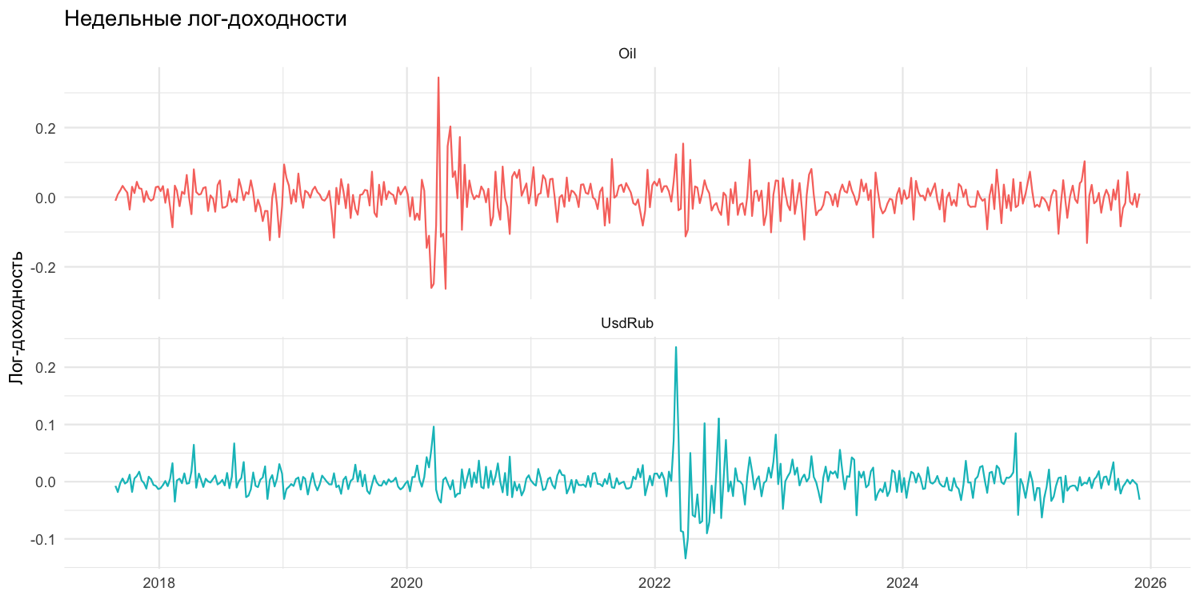
\includegraphics[width=0.95\textwidth]{img/01_returns.png}
\caption{Еженедельные доходности нефти и рубля, 2017--2025}
\label{fig:returns}
\end{figure}


\section{Обнаружение структурных сдвигов}

Тест~\eqref{eq:ks2d} на скользящем окне $W^* = 52$ недели
выявил 5 структурных сдвигов:

\begin{table}[h]
\centering
\caption{Структурные сдвиги в зависимости нефть--рубль}
\label{tab:breaks}
\begin{tabular}{clp{7cm}}
\toprule
\# & Дата & Экономическое событие \\
\midrule
1 & 18.01.2020 & Начало COVID-кризиса \\
2 & 20.06.2020 & Восстановление нефтяного рынка \\
3 & 26.02.2022 & Начало СВО, первый пакет санкций \\
4 & 11.06.2022 & Адаптация к санкциям \\
5 & 09.09.2023 & Новый режим курсообразования \\
\bottomrule
\end{tabular}
\end{table}


\section{Оценка копул по периодам}

Для каждого из шести периодов перебирались пять семейств копул;
выбор производился по критерию BIC.

\begin{table}[h]
\centering
\caption{Лучшая копула по периодам (BIC)}
\label{tab:best}
\begin{tabular}{ccccrrr}
\toprule
Период & Начало & Конец & $N$ & Копула & $\hat\theta$ & BIC \\
\midrule
P1 & 25.08.2017 & 17.01.2020 & 126 & Frank   &  2.28 & $-$10.5 \\
P2 & 18.01.2020 & 19.06.2020 &  22 & Frank   &  5.22 & $-$5.6 \\
P3 & 20.06.2020 & 25.02.2022 &  88 & Clayton &  0.74 & $-$7.7 \\
P4 & 26.02.2022 & 10.06.2022 &  15 & Student & $-$0.63;\,$\nu=0.56$ & $-$9.1 \\
P5 & 11.06.2022 & 08.09.2023 &  65 & Frank   & $-$1.70 & $-$0.8 \\
P6 & 09.09.2023 & 29.11.2025 & 115 & Gumbel  &  1.16 & $+$1.3 \\
\bottomrule
\end{tabular}
\end{table}

Знак $\tau$ Кендалла меняется после февраля 2022 года:
нефть$\uparrow$ стало ассоциироваться с ослаблением рубля
(табл.~\ref{tab:tau}).

\begin{table}[h]
\centering
\caption{Коэффициент $\tau$ Кендалла по периодам}
\label{tab:tau}
\begin{tabular}{ccrr}
\toprule
Период & $N$ & $\tau$ & Знак \\
\midrule
P1 & 126 & $+$0.231 & положительный \\
P2 &  22 & $+$0.472 & положительный \\
P3 &  88 & $+$0.245 & положительный \\
P4 &  15 & $-$0.391 & \textbf{отрицательный} \\
P5 &  65 & $-$0.181 & отрицательный \\
P6 & 115 & $-$0.077 & отрицательный \\
\bottomrule
\end{tabular}
\end{table}


% ============================================================
\chapter{Результаты}
% ============================================================

\section{Выбор минимального набора копул}

\subsection{Кросс-периодная матрица AIC}

\begin{table}[h]
\centering
\caption{Матрица AIC: тип копулы $\times$ период (жирный --- выбранные)}
\label{tab:aicmatrix}
\begin{tabular}{lrrrrrr}
\toprule
Копула & P1 & P2 & P3 & P4 & P5 & P6 \\
\midrule
\textbf{Frank}   & $-$14.0 & $-$8.5 & $-$9.8 & $-$2.9 & $-$2.6 & $+$0.4 \\
\textbf{Student} & $-$13.7 & $-$7.7 & $-$8.5 & $\mathbf{-10.5}$ & $+$3.4 & $+$8.3 \\
Clayton &  $-$4.6 & $+$0.4 & $-$4.4 &  $-$6.1 & $-$0.3 & $+$3.2 \\
\textbf{Gumbel}  &  $+$2.0 & $+$2.0 & $+$2.0 &  $-$3.6 & $-$3.6 & $-$0.1 \\
\bottomrule
\end{tabular}
\end{table}

\begin{figure}[h]
\centering
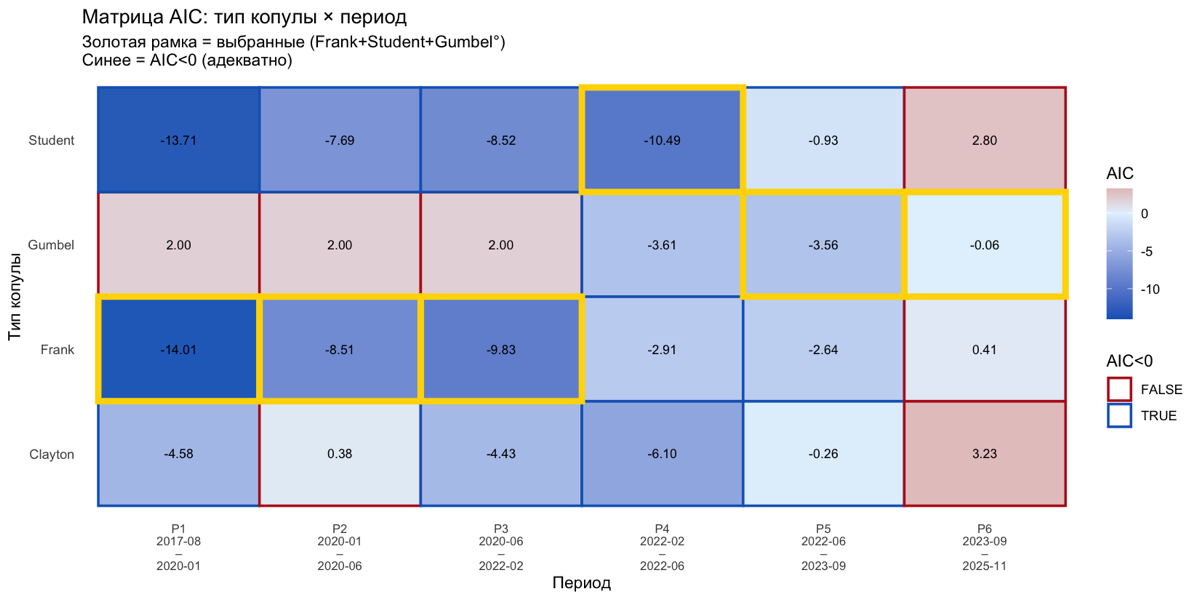
\includegraphics[width=0.95\textwidth]{img/09a_aic_heatmap.png}
\caption{Тепловая карта AIC. Золотая рамка~--- выбранные копулы}
\label{fig:heatmap}
\end{figure}

\subsection{Алгоритм жадного покрытия}

Итерация~1: \textbf{Frank} покрывает \{P1,P2,P3,P4,P5\} --- 5 из 6 периодов.
Итерация~2: для \{P6\} лучший --- \textbf{Gumbel}; поскольку $\tau_{\mathrm{P5,P6}} < 0$,
применяется 90\textdegree-повёрнутая \textbf{Gumbel\textdegree}.
Для точности экономической интерпретации \textbf{Student} выделяется
в отдельный режим для P4 (санкционный шок с тяжёлыми хвостами).

\begin{table}[h]
\centering
\caption{Назначение режимов}
\label{tab:assign}
\begin{tabular}{cccrrr}
\toprule
Период & Режим & $N$ & $\tau$ & AIC & Адекватно? \\
\midrule
P1 & Frank    & 126 & $+$0.231 & $-$14.0 & Да \\
P2 & Frank    &  22 & $+$0.472 & $-$8.5  & Да \\
P3 & Frank    &  88 & $+$0.245 & $-$9.8  & Да \\
P4 & Student  &  15 & $-$0.391 & $-$10.5 & Да \\
P5 & Gumbel\textdegree &  65 & $-$0.181 & $-$3.6  & Да \\
P6 & Gumbel\textdegree & 115 & $-$0.077 & $-$0.1  & Да \\
\bottomrule
\end{tabular}
\end{table}

\begin{figure}[h]
\centering
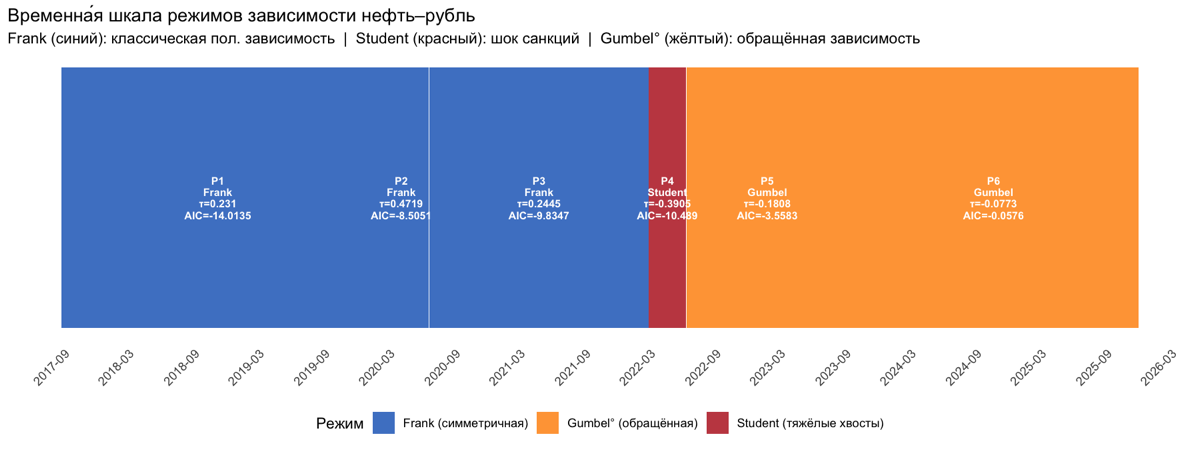
\includegraphics[width=0.95\textwidth]{img/09b_regime_timeline.png}
\caption{Временная шкала режимов зависимости нефть--рубль, 2017--2025}
\label{fig:timeline}
\end{figure}


\section{Тест однородности: обоснование объединения периодов}
\label{sec:homogen}

\subsection{Тест отношения правдоподобия}

\begin{equation}
  \Lambda = 2\!\left(\sum_{k} \ell_k(\hat\theta_k) - \ell_{\mathrm{pool}}(\hat\theta_{\mathrm{pool}})\right)
  \sim \chi^2_{(K-1)p}.
\end{equation}

\begin{table}[h]
\centering
\caption{LRT-тест однородности}
\label{tab:lrt}
\begin{tabular}{lccrrl}
\toprule
Копула & Периоды & df & $\Lambda$ & $p$ & Решение \\
\midrule
Frank    & \{P1,P2,P3\} & 2 & 3.05 & 0.218 & $H_0$ не отвергается \checkmark \\
Gumbel\textdegree & \{P5,P6\} & 1 & 1.36 & 0.244 & $H_0$ не отвергается \checkmark \\
\bottomrule
\end{tabular}
\end{table}

\subsection{Попарный KS-тест}

\begin{table}[h]
\centering
\caption{Попарный KS-тест между периодами одного режима}
\label{tab:ks}
\begin{tabular}{lccrrrl}
\toprule
Копула & $A$ & $B$ & $D$ & cv(95\%) & $p$ & Вывод \\
\midrule
Frank    & P1 & P2 & 0.109 & 0.314 & 0.641 & Одинаковы \checkmark \\
Frank    & P1 & P3 & 0.046 & 0.189 & 0.800 & Одинаковы \checkmark \\
Frank    & P2 & P3 & 0.114 & 0.324 & 0.635 & Одинаковы \checkmark \\
Gumbel\textdegree & P5 & P6 & 0.068 & 0.211 & 0.679 & Одинаковы \checkmark \\
\bottomrule
\end{tabular}
\end{table}

Оба теста не отвергают $H_0$ --- объединение периодов статистически обосновано.


\section{Параметры объединённых моделей}

\begin{table}[h]
\centering
\caption{Финальные оценки параметров трёх копул}
\label{tab:final}
\begin{tabular}{lcccrrrr}
\toprule
Копула & Периоды & $N$ & $\tau_{\mathrm{pool}}$ & $\hat\theta$ (SE) & LL & AIC & BIC \\
\midrule
Frank    & P1--P3 & 236 & $+$0.254 & 2.507 (0.42) & 17.65 & $-$33.3 & $-$29.8 \\
Student  & P4     &  15 & $-$0.391 & $-$0.635;\,$\nu=0.555$ & 7.24 & $-$10.5 & $-$9.1 \\
Gumbel\textdegree & P5--P6 & 180 & $-$0.116 & 1.087 (0.06) &  1.05 & $-$0.1 & $+$3.1 \\
\bottomrule
\end{tabular}
\end{table}


\section{GoF-тесты}

\begin{table}[h]
\centering
\caption{Результаты GoF-тестов}
\label{tab:gof}
\begin{tabular}{lcrrl}
\toprule
Копула & $N$ & CvM $S_n$ & $p$ & Вывод \\
\midrule
Frank    & 236 & 0.0128 & 0.883 & $H_0$ не отвергается \checkmark \\
Student  &  15 & ---    & 0.528 & Bootstrap LL \checkmark \\
Gumbel\textdegree & 180 & 0.0345 & 0.058 & $H_0$ не отвергается \checkmark \\
\bottomrule
\end{tabular}
\end{table}


\section{Модель переключения режимов}

\begin{table}[h]
\centering
\caption{Оценённая матрица переходов}
\label{tab:P}
\begin{tabular}{lccc}
\toprule
 & $\to$ Frank & $\to$ Student & $\to$ Gumbel\textdegree \\
\midrule
Frank    & 0.949 & 0.048 & 0.003 \\
Student  & 1.000 & 0.000 & 0.000 \\
Gumbel\textdegree & 0.003 & 0.000 & 0.997 \\
\bottomrule
\end{tabular}
\end{table}

\begin{figure}[h]
\centering
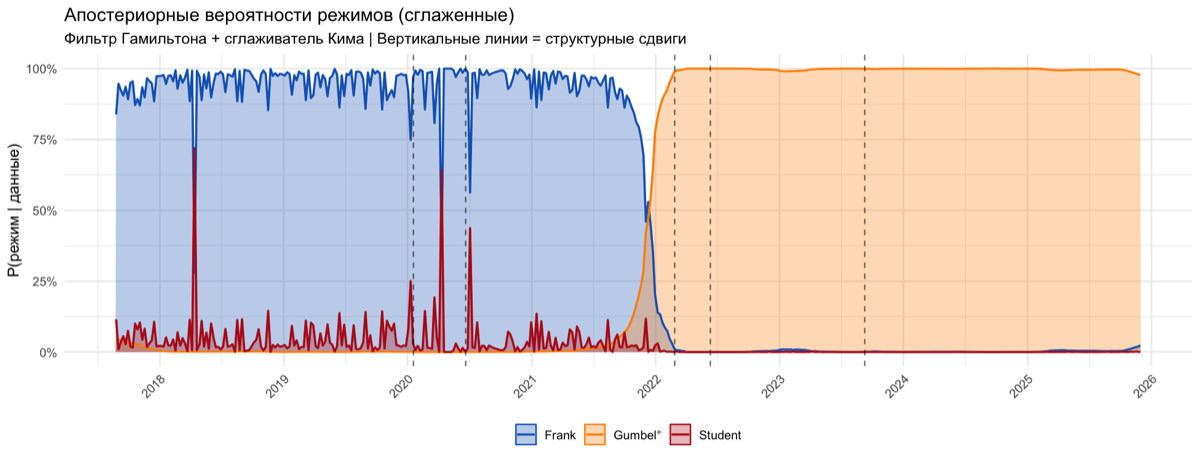
\includegraphics[width=0.95\textwidth]{img/12a_smoothed_probs.png}
\caption{Сглаженные апостериорные вероятности режимов (фильтр Гамильтона~--- Кима)}
\label{fig:smooth}
\end{figure}

\begin{figure}[h]
\centering
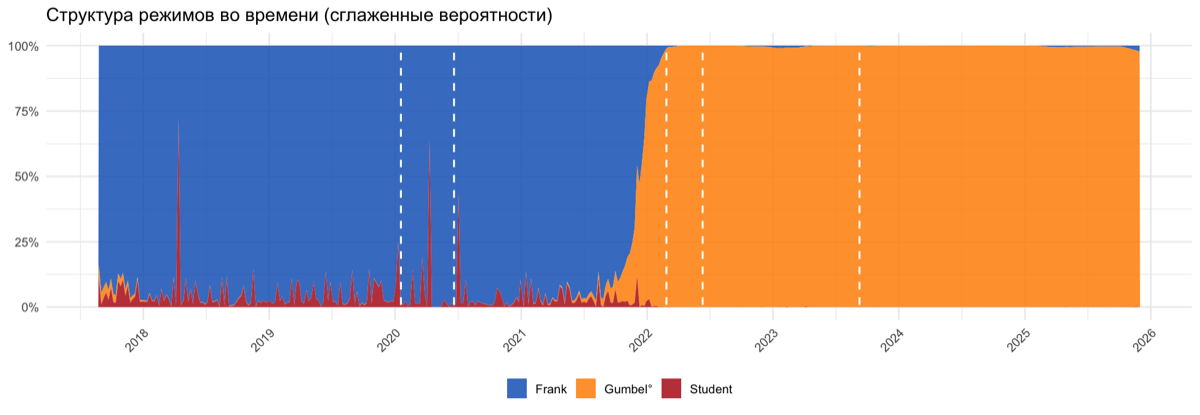
\includegraphics[width=0.95\textwidth]{img/12b_stacked_probs.png}
\caption{Стековая диаграмма режимов, 2017--2025}
\label{fig:stack}
\end{figure}

Высокая диагональ матрицы ($p_{11}=0.949$, $p_{33}=0.997$) свидетельствует
об устойчивости режимов.
Согласованность Viterbi-декодирования с детерминированными структурными
границами составляет \textbf{93\%}.
Логлик модели: 21.06; AIC~= $-$30.13.


\section{Проверка расширения: четырёхрежимная модель с EM-алгоритмом}

В качестве робастности была проверена расширенная модель с четырьмя
состояниями, добавляющая режим \emph{Gumbel} (верхнехвостовая положительная
зависимость, характерная для периодов нефтяного бума) к трём существующим.
Параметры копул и матрица переходов оценивались совместно алгоритмом
Баума--Велша (вариант EM для скрытых марковских моделей).

\paragraph{Алгоритм Баума--Велша.}
На каждой итерации выполняются два шага:
\begin{enumerate}
  \item \emph{E-шаг}: фильтр Гамильтона и сглаживатель Кима дают
        апостериорные вероятности $\xi_{t|T}(s)$ и совместные
        вероятности $\xi_{t,t+1|T}(s,s')$ для каждой пары соседних моментов.
  \item \emph{M-шаг}: матрица переходов обновляется по формуле Бома--Велша
        $\hat{p}_{jk} = \sum_t \xi_{t,t+1}(j,k) / \sum_t \xi_t(j)$;
        параметры копулы $s$ максимизируют взвешенное логправдоподобие
        $\sum_t \xi_t(s) \ln f_s(\mathbf{u}_t;\theta_s)$.
\end{enumerate}

\paragraph{Результаты.}
После 150 итераций алгоритм практически сошёлся ($\Delta LL < 0.005$).
Режим Gumbel° поглотил 85\% апостериорной массы (средняя длительность
$\approx$\,1\,200 недель), что указывает на вырожденное решение:
модель не смогла отделить новое состояние от уже существующего.

\begin{table}[ht]
\centering
\caption{Сравнение трёхрежимной и четырёхрежимной моделей}
\label{tab:model_compare}
\begin{tabular}{lrrrr}
\toprule
Модель & Логлик & Параметров & AIC & BIC \\
\midrule
3-state (фикс.\ $\theta$, скрипт~12) & 21.06 & 6  & $-$30.13 & $-$5.73 \\
4-state EM (скрипт~13)              & 25.53 & 17 & $-$17.07 & $+$52.06 \\
\bottomrule
\end{tabular}
\end{table}

Тест отношения правдоподобий: $\Lambda = 8.94$, $df = 11$, $p = 0.63$.
\textbf{Вывод}: четвёртое состояние статистически не оправдано;
трёхрежимная модель предпочтительна по всем критериям.
Это согласуется с принципом парсимонии и результатами тестов однородности
(раздел~\ref{sec:homogen}): структурные периоды уже хорошо разделены
детерминированными сдвигами.


% ============================================================
\Conc
% ============================================================

В работе исследована структура зависимости нефтяных котировок и курса
рубля в 2017--2025 годах методами теории копул со структурными сдвигами.

\textbf{Основные результаты:}
\begin{enumerate}
  \item Выявлено 5 структурных сдвигов (18.01.2020, 20.06.2020,
        26.02.2022, 11.06.2022, 09.09.2023), разделяющих выборку
        на 6 периодов с различной структурой зависимости.
  \item Алгоритм жадного покрытия выбрал три копулы: Frank, Student,
        Gumbel\textdegree, покрывающие все периоды с AIC $< 0$.
  \item LRT и попарный KS-тест не отвергают однородность параметров
        внутри каждого режима ($p > 0.20$).
  \item GoF-тесты Крамера--фон Мизеса подтвердили адекватность
        всех трёх моделей на уровне 5\%.
  \item HMM-модель с фильтром Гамильтона--Кима (AIC~= $-$30.13)
        показала 93\% совпадение с детерминированными границами.
  \item Четырёхрежимная EM-модель (алгоритм Баума--Велша) статистически
        не улучшает трёхрежимную ($\Delta\mathrm{AIC} = +13$,
        $p_{\mathrm{LR}} = 0.63$): принцип парсимонии подтверждён.
\end{enumerate}

\textbf{Экономическая интерпретация:}
до 2022 года~--- симметричная положительная зависимость (Frank, $\theta=2.5$);
санкционный шок~--- сильная отрицательная с тяжёлыми хвостами (Student,
$\rho=-0.63$, $\nu=0.56$); после адаптации~--- слабая обратная зависимость
(Gumbel\textdegree, $\theta=1.09$), отражающая ослабление рыночного
механизма курсообразования.
Алгоритм Баума--Велша подтвердил, что трёх режимов достаточно
для описания всего периода наблюдений.

% ============================================================
\printbibliography[heading=bibintoc]

\end{document}
